%% LaTeX2e class for student theses
%% sections/content.tex
%% 
%% Karlsruhe Institute of Technology
%% Institute for Program Structures and Data Organization
%% Chair for Software Design and Quality (SDQ)
%%
%% Dr.-Ing. Erik Burger
%% burger@kit.edu
%%
%% Version 1.3.2, 2017-08-01

\chapter{Motivation}
The \textit{Worldwide LHC Computing Grid (WLCG)} is one of the largest grids in the world and processes the data created by the \textit{Large Hadron Collider (LHC)} at CERN \cite{wlcg_update}. However, there is no model or simulation existing to evaluate the load balancing strategies of the grid.

The following chapter describes the WLCG in detail, the current state of the load balancing, and the desired state in the future.

\section{Worldwide LHC Computing Grid}

The WLCG processes 50 Petabytes of data each year, created by the LHC at CERN \cite{data_process}. 
With its help the \textit{Higgs boson} was discovered in 2012 \cite{wlcg_online}.

The grid consists of 170 computing centres distributed in 42 countries. Combined it has 72.000 CPUs, 386 Petabytes online data space and 368 Petabytes nearline space (tape) \cite{wlcg_data}. Every day it runs 2 million jobs.

At CERN there are four experiments, namely: Atlas, Alice, CMS, LHCB. They all use the grid in a similar way, but not the same \cite{wlcg_computing}. The WLCG is structured into three Tiers, which are described in \ref{fig:wlcg}. Tier 0 is the CERN compute centre, which stores all raw data of the experiments, makes the first pass reconstruction and distributes raw data to T1 compute centres. Tier 1 consists of 13 sites, which store a share of raw and reconstructed data. Tier 2 sites, which are mostly located at universities or other scientific institutes, do monte carlo production. In contrast to Tier 1 sites, the Tier 2 sites do not have much storage.

The WLCG is heterogeneous, meaning one site has different resources than an other site, the network connections between sites vary, and even the nodes in one site have different resources. It is trending to use more virtualization, resulting in even more heterogeneity \cite{wlcg_update}.

Our work will focus on modelling and simulating load balancing strategies of the CMS experiment, but because the experiments use the grid in a similar way, the results of our work can be presumably transferred to the other experiments.

	\begin{figure}
		\centering
		\includegraphics[width=0.6\linewidth]{images/WLCG}
		\caption[]{Tier structure of WLCG \cite{wlcg_tiers}}
		\label{fig:wlcg}
	\end{figure}
	

\section{Current State}
Currently the load balancing strategy of the WLCG is not optimal, e.g. it does not account the nature of the jobs. There are io-heavy jobs and compute-heavy jobs, if this nature is not accounted, it leads to a bad utilization of the nodes. It is desired, that the right amount of io-and compute-jobs are submitted to a site, so resulting in a good utilisation of IO and CPU. 

HTCondor is the batchsystem, which is used for the WLCG and is the central point for the load balancing.
It not only decides on which site the job should run, but even on which node, so it has full control over the load.

There are several other ideas how to improve the CMS computing model, but without a simulation no one can evaluate which one is best in terms of speed-up, cost or utilization.


\section{Outlook}
The amount of data produced by the LHC increases steadily, thus more computing resources are needed.
However, these resources will not increase in the same magnitude as the produces data, thus better utilization of the given resources is required. Our approach will allow to simulate the effects of different load balancing strategies and decide on these results what the best strategy is. The scheduling problem itself is np complete, so the optimal solution will not be found, but we can decide on a set of strategies which one is the best \cite{1698650}.

Further, our approach can be used to evaluate the effects of changing the grid. Thus, we can decide what the best approach is to improve the CMS computing model, e.g. adding cache, create a new network connection or allow dynamic nodes.
This is hard to decide without simulation, because one cannot consider all side-effects, e.g. increasing the CPU resources may be useless, because then the network could become the bottleneck.

\chapter {Foundations}
In this chapter \textit{Palladio} is described, which is intended to be used as the tool to model and simulate the CMS computing model.
An other important foundation is to explain what the differences between grids and clouds are.

\section{Palladio}
Palladio is a software architecture simulator developed by Karlsruhe Institute of Technology (KIT), FZI Research Center for Information Technology, and University of Paderborn. The development started 2003 and it is still actively developed today. Palladio predicts quality of software properties (e.g. performance) using several models of a system \cite{BECKER20093}.

These models are the component model, the assembly model, the resource model, the allocation model, and the usage model.
The component model specifies the structure and behaviour of the components independently from their later usage. This allows reuse of the components,  but requires its parametrization.
The assembly model specifies how the components are connected to model the software architecture. 
The resource model  describes the resources environment.
The allocation model describes how the different components are mapped to the resources.
Finally, the usage model describes how the system is used  \cite{BECKER20093}.

After these models are created, Palladio can be used to simulate the system, choosing one of several supported simulators. This process is shown in \ref{fig:palladio}. 

Palladio was extended with the \textit{architectual templates} to make it possible to model cloud computing environments efficiently \cite{arch}.

SimuLizar is another simulator for Palladio to simulate self-adaptive systems \cite{becker2013simulizar}. It was later extended to support the metrics scalability, elasticity, and efficiency \cite{arch}.

The first case studies using Palladio in cloud environments show that the results are accuracy \cite{arch}. However, Palladio was never used to model and simulate such a large system as the CMS computing model.

\begin{figure}
	\centering
	\includegraphics[width=0.9\linewidth]{images/palladio}
	\caption[]{Process of Palladio \cite{BECKER20093}}
	\label{fig:palladio}
\end{figure}



\section{Differences Grid-Computing and Cloud-Computing}
Grid-computing are distributed systems working together to solve a problem. Cloud-computing has a lot in common with grid-computing, because it is also a distributed system working together and because it evolved from grid-computing \cite{foster2008cloud}.
However, there are also some important differences.

Some of the key aspects are: virtualization, on-demand resource provisioning, and elasticity \cite{foster2008cloud}.
Firstly, cloud-computing uses massively virtualization, this means that assigning application models to computing nodes do not model the abstraction correctly TODO \cite{cloud_sim}. Secondly, the cloud allows on-demand resource provisioning \cite{foster2008cloud}. Further, clouds are elastic, they scale up or down according to the currently required resources and allow autoscaling of applications, meaning the provisioned resources to an application are dynamically changed \cite{cloud_sim}.

\chapter{State of the Art}
\label{state}
There are a lot other approaches beside Palladio that deal with the simulation of grids or clouds.
In this chapter a selection of these is presented.


\section{Grid Simulators}
Grid simulators exist since the late 1990s, the most ones have been created in the mid 2000s. However, most simulators are not developed any more. In this section the most common ones are presented.

\subsection{SimGrid}
\label{simgrid}
SimGrid is a framework for large-scale distributed systems and one of the earliest created grid simulators \cite{simgrid_update}. Its first release was 1998 and is one of the few that is still developed today.
Further, its one of the most used simulators \cite{simgrid_update}.

In SimGrid one has to define the platforms, and the Deployment in XML and the application and scheduling in C. It supports simulation of CPU, I/O, and network resources, heterogeneous workloads and heterogeneous platforms \cite{simgrid_update}.

It is more scalable than GridSim, which is an other popular grid simulator \cite{simgrid_update}.
\ref{diag} shows the simulation time of SimGrid and GridSim for 2000 nodes and increasing tasks.
SimGrid performs significantly better that GridSim, because GridSim´s simulation time increases quadratic with the number of tasks, while SimGrid´s only increases linear. At 500.000 tasks GridSim requires more than one hour and 4.4 GiB of memory to simulate, while SimGrid needs less than 14 seconds and with only 165 MiB.

This performance difference is created by a lot of optimizations, including implementing light-weight execution contexts, using lazy activity updates, and using trace integration for resource management \cite{simgrid_update}.

\begin{center}

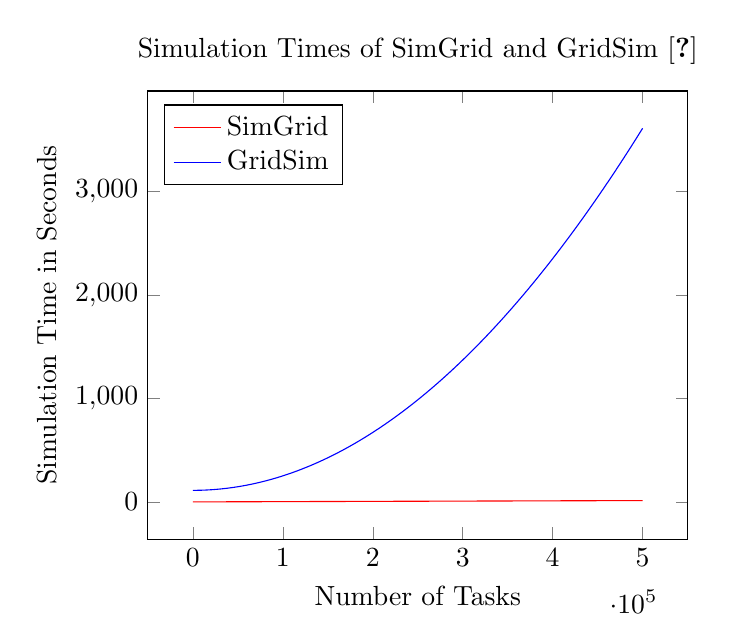
\begin{tikzpicture}
\label{diag}
\begin{axis}[
legend pos=north west,
title=Simulation Times of SimGrid and GridSim \cite{simgrid_update},
xlabel={Number of Tasks},
ylabel={Simulation Time in Seconds},
legend entries={SimGrid, GridSim},]
\addplot [red, domain=1:500000, samples=1000] {0.1*10^(-3)*2000+26*10^(-6)*x};
\addplot [blue, domain=1:500000, samples=1000] {56*10^(-3)*2000+14*10^(-9)*x^2};

\end{axis}
\end{tikzpicture}
\end{center}


\subsection{GridSim}
\label{gridsim}

GridSim was created 2001 as part of the gridbus project and was developed until 2010 \cite{gridsim}.
It is focused on evaluating scheduling and resource brokering \cite{al2012simulation}.
It supports simulation of CPU, I/O and network resources, heterogeneous workloads and heterogeneous platforms \cite{gridsim}. Its implemented in Java, using SimJava´s discrete event simulation  \cite{gridsim}.
It is popular and has been used from other members of the community. 

However, as in section \ref{simgrid} mentioned, it does not scale very well and further it does not deliver realistic results regarding moving or the storage of data \cite{1698650} .

\subsection{GangSim}

GangSim derived from an enhancement of Ganglia monitoring toolkit in 2005 \cite{dumitrescu2005gangsim}. It was not further developed after its initial release.
It is used to handle usage constraints for sites and virtual organizations. It evaluates allocation of individual resource from the interactions between allocation policies across virtual organisations \cite{dumitrescu2005gangsim}.

It supports simulation of CPU, I/O and network resources, heterogeneous workloads and heterogeneous platforms \cite{dumitrescu2005gangsim}.

In difference to most other simulators, it is a discrete time-stepped simulators \cite{dgsim}. This means it will simulate every time-step, even if nothing happens. This results in a bad performance and bad scalability.



\subsection{OptorSim}
OptorSim was created 2003 as part of the European Data Grid project and is used to evaluate data replication strategies in grids \cite{optorsim}. To do that it simulates the time needed to copy or access the required files for each job and replicating files according to a given strategy.

It is not developed any more and does not consider job scheduling optimization. Because of its little scope, it does not support simulating of CPU and I/O resources, and heterogeneous platforms \cite{optorsim}.


\subsection{DGSim}
To improve the simulation environments the DGSim framework focuses on automating and optimizing the overall simulation process \cite{dgsim}. It helps setting up the experiment by to generating realistically grids, generate grid dynamics and evolution events, and generate realistic grid workload or use traces of existing ones. Further, it enables grouped or batches of simulations \cite{dgsim}.

It was created in 2007 at Delft University of Technology, and is not public available, so nobody else used it.


\subsection{ChicagoSim}
The data locality is a important aspect in grid computing, thus ChicagoSim was created in 2003 to evaluate differnt scheduling and data replication algorithms \cite{chicagosim}. In contrast to OptorSim it also evaluates scheduling algorithmns. 
One of the results is that scheduling jobs to sites containing the data and replicating popular data-sets is a good solution and works better than scheduling jobs to idle processors and moving the data.

ChicagoSim was not further developed, it does not support simulating CPU or I/O, instead simple constant waiting time is used, without any concurrence to resources \cite{chicagosim}. 



\section{Cloud Simulators}
In the recent years the research went from grid simulators to cloud simulators, because grid simulators cannot sufficiently model the cloud infrastructure \cite{compare_grid_cloud}. Although the WLCG is a grid and therefore a grid simulator would be more suitable that an cloud simulator, it is useful to know about the latest developments in cloud simulators. Therefore this sections presents a brief overiew about the most common simulators.

\subsection{CloudSim}
CloudSim is the most used and most sophisticated cloud simulator \cite{compare_grid_cloud}. Created 2010 at the University of Melbourne as part of the cloudbus project. It is based on GridSim and itself is the foundation for a lot of other simulators. It shows a good scalability, simulation 100.000 machines in less than 5 min, requiring only 75 MB of RAM \cite{survey_clouds}. It supports both system and behaviour modelling of cloud system components such as data centers, virtual machines and resource provisioning policies.

It was later extended with a network simulation component to evaluate applications which communicate \cite{networkcloudsim}.

\subsection{CDOSim}
CDOSim is simulator based in CloudSim with the purpose to evaluate competing cloud deployment options (CDOs) \cite{cdosim}.  It was developed 2012 at Kiel University. It represents more user than provider perspective and hide fine fine-grained internals of a cloud platform. It helps to find best ratio between high performance and low costs, by helping to  select a cloud provider, the mapping between service and virtual machines and adaption strategies. 

\subsection{LocalitySim}
Another simulator based on CloudSim is LocalitySim, which was created 2016 at the University of Cairo \cite{localitysim}. Data locality affects the performance of any scheduling algorithm. If the scheduler places the job far away from its data, extra time is needed to transfer data. Most other cloud simulators are not supporting data locality.


\subsection{GreenCloud}

GreenCloud focuses on the energy efficiency of clouds \cite{green_cloud}. It was created 2012 
at the University of Luxembourg. It focuses specifically on the measurement of energy consumption of severs, switches and links. It simulates the network on packet level, because of this it network model is very accurate.  

However, it assumes that every server only has a single core and virtualization, storage area networks and resource management are not considered \cite{survey_clouds}.


\subsection{Cloud Autoscaling Simulation}
Researches at the Czech Technical University tried to evaluate predictive autoscaler, but found that CloudSim had accuracy and speed issues \cite{autoscale_cloud}. Thus, they implemented a new simulation method based on queueing models, delivering realistic results. 

They found out that the autscaling is very stable and cost-efficient when they scale up based on latency and scale down based on utilization. 

\section{The MONARC Project}
The MONARC project was started 1998 to help with the inital design of the WLCG at CERN \cite{monarc2000models}. They created models and simulations of possible structures of the grid. For that the MONARC simulator was developed. 
The results indicated that a hierarchical structure with regional centers would perform best, thus we have the 3 Tier structure today \cite{morita2001validation}.

2006 a second version of the MONARC simulator was released, which is not only usable for the WLCG but general large scale distributed computing systems \cite{legrand2003monarc}. But one clearly see that its origin is WLCG. In difference to its first version a discrete-event approach instead of a discrete time-stepped was used.

2010 Zach et al. \cite{1742-6596-331-7-072038} used MONARC2 to simulate the ALICE Tier-2 site in Prague. The simulation included 3000 CPUs, and the CPU, network and I/O resources were simulated. The results are accurate, however they could not simulate the network load correctly and MONARC2 already ran into performance issues, making it not usable for even larger systems.


\section{CACTOS}
CACTOS is a approach to cloud infrastructure automation and optimization \cite{cactos}. It includes the 
CACTOS Runtime Toolkit for monitoring and resource management and the CACTOS Prediction Toolkit for evaluation of alternative data center deployment scenarios, and resource management algorithms.
The predication toolkit is built on Palladio and SimuLizar.
The models of the predication toolkit regarding resources or application behaviour is updated using monitoring data, this is done to handle the highly dynamic behaviour of clouds. F. Pop et al. \cite{1698650} suggested the idea to couple monitoring and grid simulation tools in 2006.

CACTOS supports the rapid testing of resource management algorithms due the ability to simulate them without reimplementing them for the Prediction Toolkit and automatic creation of workload models by using runtime monitoring data.\cite{rapidtesting}. 

First case studies show that the predication toolkit has a high accuracy, but it was not tested on a large system yet \cite{rapidtesting}.




\chapter{Discussion}
\label{dis}
Several grid and cloud simulators have been presented in chapter \ref{state}. Grid simulators are a better option for modelling and simulating the CMS computing model, see section \ref{diff}] for the differences of grid and cloud computing. It may be possible to use a cloud simulator, but the added functionality may give an overhead and to model a grid in cloud may be needed workaround and the result would not be as easy to understand. For cloud simulators CloudSim is the most evolved one.

Table \ref{compare} compares the grid simulators based on our needs. As one can see only SimGrid and Palladio do full fill them, but Palladio its not clear if its as scalable as needed.  As part of the CACTOS project Palladio and SimuLizar are made ready to use for cloud, thus we expect that it will scale. All other simulators are either not developed any more, have never been intended to be used as a general simulater, and have only be created to research one small aspect. Most simulators support the simulation of CPU, I/O and network ressources. Also heterougnous platforms and tasks are supported.

As mentioned in \ref{state} OptorSim, ChicagoSim and LocalitySim are the only simulators which consider data locality. However, this feature is not needed for simulating load balancing strategies, because we only need to effects of a data replication strategy, e.g. reduce data miss rate 30\%. The data locality feature is needed if one wants to evaluate a better data replication strategies. 

There was no indication that a similar big grid or cloud as the CMS computing grid was simulated yet, so our work will evaluate if the existing tools make it possible to do it.


\begin{center}
\label{compare}
\captionof{table}{Comparison of Grid Simulators} 
\scalebox{0.9}{
\begin{tabular}{|c|c|c|c|c|c|c|c|c|c|}
	\hline
	\rot{Simulator} & \rot{Active Project} & \rot{General usable} & \rot{Scheduling} & \rot{CPU} & \rot{I/O} & \rot{Network} & \rot{Heterogeneous Platforms  } & \rot{Heterogeneous Tasks} & \rot{Scalable} \\
	\hline
	SimGrid & \cmark&\cmark&\cmark&\cmark&\cmark&\cmark&\cmark&\cmark&\cmark\\
	\hline
	GridSim & \xmark&\cmark&\cmark&\cmark&\cmark&\cmark&\cmark&\cmark&\xmark\\	
	\hline
	GangSim & \xmark&\xmark&\cmark&\cmark&\cmark&\cmark&\cmark&\cmark&\xmark\\	
	\hline
	OptorSim & \xmark&\xmark&\xmark&\xmark&\xmark&\cmark&\xmark&\cmark&\qmark\\	
	\hline
	DGSim & \xmark&\xmark&\cmark&\xmark&\cmark&\cmark&\cmark&\cmark&\cmark\\	
	\hline
	ChicagoSim & \xmark&\xmark&\cmark&\xmark&\xmark&\cmark&\cmark&\cmark&\cmark\\	
	\hline
	MONARC & \xmark&\cmark&\cmark&\cmark&\cmark&\cmark&\cmark&\cmark&\xmark\\	
	\hline
	Palladio & \cmark&\cmark&\cmark&\cmark&\cmark&\cmark&\cmark&\cmark&\qmark\\	
	\hline

\end{tabular}
}
\end{center}

\chapter{Conclusion}

It was shown that Palladio is a good choice to start with the modelling and simulation of the load balancing strategies of the CMS experiment. An other good candiate is SimGrid. However, if it shows that Palladio is not scalable enough, we can transform our models to SimGrid models using model-to-model transformation and use it to simulate. Also we keep CloudSim in mind, because good cloud simulater for big systems. 

Futher, it was shown that the CMS computing experiment was not simulated, nor other large grid or cloud was simulated. Our work will make a simulation magnitudes larger than existing,  and show if the existing simulators can be used.

\chapter{Outlook}
We will first start to use Palladio to model and simulate the Tier 1 computing centre GridKA. 
For this Performance log have to be ausgewartet, the model be created, and validated.
We then use this as foundation to model the whole CMS computing model.

